\chapter{Scene Graphs}

\section{Mathematical Description}
We model the geometric state of a scene at a single time point as a \emph{scene graph}, which is a tuple $(G, \Theta, Z)$, where $G = (V, E)$ is a directed tree that encodes the scene graph \emph{structure} and $\Theta$ encodes the scene graph \emph{continuous parameters} and $Z$ encodes the scene graph \emph{discrete parameters}.
Although the framework we present can represent articulated objects, in this paper we only consider scenes involving a set of rigid objects $O$.
The scene graph structure includes a vertex $v_o \in V$ for each object $o \in O$ that represents the 6DoF pose of object $o$, as well as a vertex $r \in V$ that represents the the coordinate frame of the observer.
A directed edge $e = (v_i, v_j) \in E$ between objects $i, j \in O$ encodes that the pose of object $j$ is parametrized \emph{relative to} the pose of object $i$, by parameters $\theta_e$ and $z_e$.
The pose of object $j$ relative to object $i$ is denoted $\Delta x(z_e, \theta_e) \in SE(3)$.
A directed edge $e = (r, v_j) \in E$ from the root to an object $j \in O$ encodes that the pose of object $j$ is not parametrized relative to that of any object, but is instead a full 6DoF pose $\theta_e \in SE(3)$ where $SE(3)$ is the special Euclidean group consisting of all 6DoF poses.
The continuous and discrete parameters of the scene graph consist of the parameters for each edge in the structure ($\Theta := \{\theta_e\}_{e \in E}$ and $Z := \{z_e\}_{e \in E}$).
The set of edges $E$ must \emph{span} the set of vertices $V := \{r\} \cup \{v_o\}_{o \in O}$; that is the scene graph structure $G$ is a \emph{directed spanning tree}.

\subsection{Computing the 6DoF poses of all objects in the scene} \label{6dofCalculation}
Given a scene graph $(G, \Theta, Z)$ the pose $x_i \in SE(3)$ of an object $i \in O$ relative to the observer coordinate frame can be computed by walking path in the tree $G$ from the root vertex $r \in V$ to the vertex $v_i \in V$, and successively computing the pose of each object along the path from the pose of its parent (the set of all such poses is $X := \{x_i\}_{i \in O}$.
That is, given pose $x_u \in SE(3)$ and edge $(u, v) \in E$, the pose $x_v \in SE(3)$ is computed as $x_v := x_u \cdot \Delta x(z_e, \theta_e)$ where $\Delta x(z_e, \theta_e) \in SE(3)$ is the relative pose between vertex $u$ and vertex $v$.
For an edge from the root vertex to an object vertex ($e = (r, v_i)$), $x_u := \mathbf{1}$ (the identity element of $SE(3)$) and $\Delta x(z_e, \theta_e) = \theta_e \in SE(3)$ (note that there are no discrete parameters in this case, so $z_e := ()$).
The functional form of $\Delta x(z_e, \theta_e)$ for an edge $e$ between two objects is discussed below.
One requirement is that $\Delta x(z_e, \theta_e)$ is a differentiable function of $\theta_e$; this enables inference algorithm that exploit gradient information.

\subsection{Modeling face-to-face contact between two objects}
An edge $(v_i, v_j) \in E$ from object $i$ to object $j$ indicates that the pose of object $j$ is represented relative to the pose of object $i$.
Various types of relative pose parametrizations for two objects are possible; for simplicity we model objects as polyhedra, and only model face-to-face contact between objects.
That is, an edge $e = (v_i, v_j)$ indicates that a face of object $i$ is in flush contact with a face of object $j$.
Since each object has multiple faces, the choice of which pair of faces is in contact is encoded in the discrete parameters $z_e$ for the edge.
Concretely, let $F_i$ and $F_j$ denote the faces of object $i$ and object $j$ respectively
Then, $z_e \in F_i \times F_j$.
The continuous parameters $\theta_e$ for an edge $e$ between two objects is an element of $\mathbb{R}^2 \times [0, 2 \pi)$ that contains two translational degrees of freedom ($s, t \in \mathbb{R}$, for the relative offset of the two faces) and one rotational degree of freedom ($\phi \in [0, 2 \pi)$).
For example, a cuboid object $i \in O$, the set of faces is $F_i = \left\{\mathrm{Top, Bottom, Left, Right, Front, Back}\right\}$.
For an edge $e = (i, j)$ where objects $i, j \in O$ where both objects $i$ and $j$ are cuboids, there are 36 possible values for $z_e$.

\paragraph{Slack variables for face-to-face contact}
We extend the parametrization of face-to-face contact between objects with three additional degrees of freedom of \emph{slack variables}: (i) one degree of freedom that encodes the perpendicular distance ($d \in [0, \infty)$) between the two contact faces, and (ii) two degrees of freedom for relative orientation of the two faces, encoded the surface normal unit vector $\mathbf{n}$ of the child object's face, relative to the parent object's face, which takes values on the sphere $S^2$.
Therefore, $\theta_e \in \mathbb{R}^2 \times [0, 2 \pi) \times [0, \infty) \times S^2$ for an edge $e = (v_i, v_j)$ between two objects $i$ and $j$.
Note that although this edge parametrization uses six degrees of freedom for object-to-object edges like the edge parametrization for edges from the root ($e = (r, v_j)$), the prior distribution on these parameters (described below) encourages object $j$ to be \emph{almost} in face-to-face contact with object $i$; whereas the prior distribution on the pose of object $j$ for an edge of the form $(r, v_j)$ is very different, and is typically a uniform distribution over positions within the scene bounding volume, and a uniform distribution on orientations.

\subsection{A Prior Distribution on Scene Graphs}  % alternative title; representation as a generative program
Various prior distributions on scene graphs are possible.
In our experiments, we use a generic prior distribution on scene graphs over a collection of objects $O$ that factors into two components:
(i) a prior distribution on scene graph structures $G$, denoted $p(G)$, and
(ii) a prior distribution on scene graph parameters $(Z, \Theta)$ given structure, denoted $p(Z, \Theta | G)$.
While uncertainty about the number of objects is possible to represent in our framework and implementation, for simplicity assume that the set of objects is known a-priori, and that there is one vertex for each object, and one vertex representing the observer coordinate frame, so $V$ is fixed a-priori to $\{r\} \cup \{v_o\}_{o \in O}$.
Therefore, $p(G)$ reduces to a prior distribution on edges in the scene graph.
For the prior distribution on structure, we use a uniform distribution on directed trees that are rooted at vertex $r$ and span all $|O| + 1$ vertices in the graph.
This set of directed trees is isomorphic to the set of undirected spanning trees over $|O| + 1$ vertices.
Therefore, the prior probability of a graph $G = (V, E)$ is obtained by using Cayley's formula to count the number of undirected spanning trees on $|O| +1$ vertices:
\begin{equation}
    p(G) := p_{\mathrm{unif}(|O|)}(G) := \left\{
    \begin{array}{ll}
    (|O| + 1)^{1 - |O|} & \mbox{if $G$ is a directed spanning tree over vertices $V$ rooted at $r$}\\
    0 & \mbox{otherwise}
    \end{array}
    \right.
\end{equation}
The prior distribution on scene graph parameters factors over the edges in the scene graph:
\begin{equation}
    p(Z, \Theta | G) := \prod_{e \in E} p_e(z_e, \theta_e)
\end{equation}
where $p_e(z_e, \theta_e)$ is a probability distribution on $z_e$ and $\theta_e$ that depends on the two vertices in the edge $e = (u, v)$.
For edges $e = (r, v_j)$ where $j$ is an object, $z_e = ()$ and $p_e(z_e, \theta_e)$ is the uniform distribution on elements of $B \times SO(3)$ where $B$ is the bounding volume of the scene and $SO(3)$ is 3D rotation group (the uniform distribution on $SO(3)$ is given by the Haar measure).
For edges $e = (v_i, v_j)$ where $i$ and $j$ are objects, recall that $z_e \in F_i \times F_j$ and (using the edge parametrization including slack variables) $\theta_e = (s, t, \phi, d, \alpha_1, \alpha_2) \in \mathbb{R}^2 \times [0, 2 \pi) \times [0, \infty) \times [0, 2 \pi)^2$.
The prior distribution on edge parameters is:
\begin{equation}
    p_e(z_e, \theta_e) := \frac{1}{|F_i| |F_j|}
    \cdot p_{\mathrm{norm}(0, \sigma)}(s) \cdot p_{\mathrm{norm}(0, \sigma)}(t)
    \cdot \frac{1}{2 \pi}
    \cdot p_{\mathrm{exp}(\beta)}(d)
    \cdot \frac{1}{2 \pi}
    \cdot \frac{1}{2 \pi}
\end{equation}
(where $p_{\mathrm{norm}}$ and $p_{\mathrm{exp}}$ are the normal and exponential distribution density functions, respectively).

\subsection{Probabilistic Dynamics on Scene Graphs}
\begin{figure}[t]
  \centering
  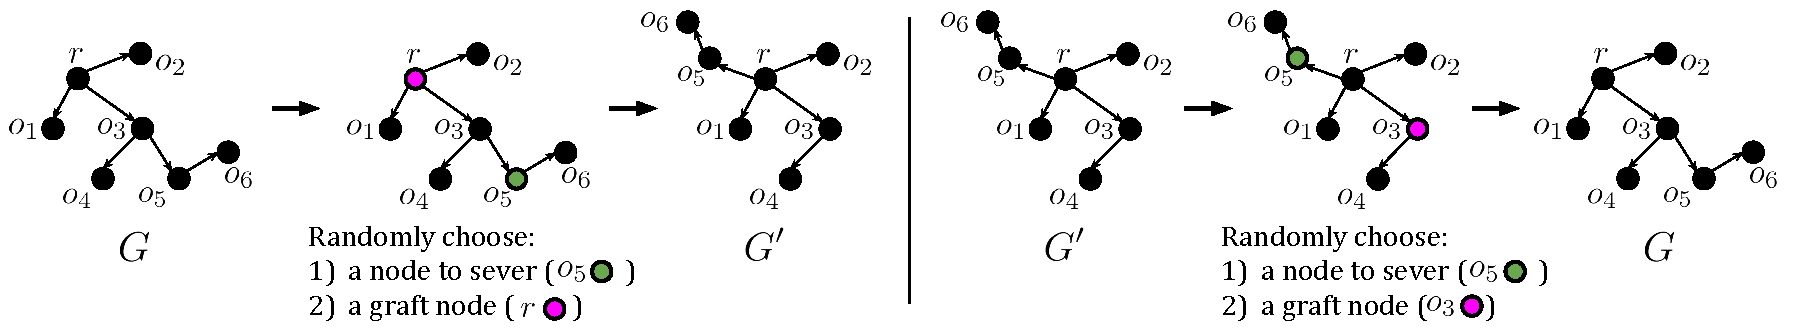
\includegraphics[width=\textwidth]{sceneGraphStructureTransition}
  \caption{
    Our random walk transition model on the structure of scene graphs modifies the spanning tree that defines the scene graph structure.
    Left: A transition from structure $G'$ to $G$ that makes $o_5$ a child of the root $r$ instead of object $o_3$.
    In $G$, parametrization of the pose of $o_5$ was previously parametrized relative to the pose of object $o_3$; in $G'$ it is parametrized independently of the pose of the other objects.
    Right: The transition on structures is reversible, and the reverse transition is unique.
    This allows us to use the transition model on structure as the basis of reversible jump MCMC moves on structure, as well within the dynamics model on structure.
  }
  \label{fig:sceneGraphS}
\end{figure}
We build temporal models of scene geometry based on Markov chains of scene graphs $\{(G_t, \Theta_t, Z_t)\}_{t=1}^T$, where $t$ indexes time, with transitions $p(G_t, \Theta_t, Z_t | G_{t-1}, \Theta_{t-1}, Z_{t-1})$.
We factor the dynamics model on scene graphs decomposes into a dynamics model on scene graph structure, and a dynamics on parameters:
\begin{align}
    p(G_t, \Theta_t, Z_t | G_{t-1}, \Theta_{t-1}, Z_{t-1}) :=
        p(G_t | G_{t-1})
        \cdot p(Z_t, \Theta_t, | Z_{t-1}, \Theta_{t-1}, G_{t-1}, G_t)
\end{align}
The dynamics on graph structure is based on a mixture of a random walk on structures (to capture incremental changes to the structure of a scene that often occur) and a uniform distribution on structures (to model sudden unexpected changes in structure):
\begin{equation}
    p(G_t | G_{t-1}) :=  0.9 \cdot p_{\mathrm{walk}}(G_t | G_{t-1}) + 0.1 \cdot p_{\mathrm{unif}(|O|)}(G_t)
\end{equation}
where $p_{\mathrm{walk}}(G' | G)$ is the distribution on graph structures induced by a sampling process in which one vertex in the undirected spanning tree is selected at random, severed from the tree, and grafted back onto the graph at a uniformly chosen vertex, subject to the condition that the resulting graph is a spanning tree;
Figure~\ref{fig:sceneGraphStructureTransition} shows an example of this process.
Recall that since the tree contains the root node $r$, this process can change the edge type $(u, v_j)$ for an object $i$ from $(r, v_j)$ (representing independent 6DoF pose) to $(v_i, v_j)$ (representing flush contact pose with another object $v_i$.
The dynamics on parameters factor according to edges in the graph:
\begin{equation}
    p(Z_t, \Theta_t | Z_{t-1}, \Theta_{t-1}, G_{t-1}, G_t) := \prod_{e \in E} p_e(z_e, \theta_e | G_t, G_{t-1}, {z_{t-1}}_e, {\theta_{t-1}}_e)
\end{equation}
If an edge $e$ is present in both $G_t$ and $G_{t-1}$, then this distribution is a mixture of a random walk and a uniform distribution.
If an edge $e$ in $G_t$ was not present in $G_{t-1}$, then this distribution is a uniform distribution.

\subsection{Robust Pose Likelihood for Modeling Noisy Object Detections}
\begin{figure}[H]
  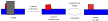
\includegraphics[width=\columnwidth]{neuralModeling}
  \caption{
    Abstract representation of our scene graph model; image data is parsed into noisy unstructured neural detections, which are modeled as observations of an underlying structured scene graph.
  }
  \label{fig:neuralModeling}
\end{figure}
Our model differs from previous inverse graphics work in an important way; while most inverse graphics pipelines create a full generative model all the way to pixel-level data, we instead model the output of a bottom-up feature detector that estimates the poses of objects from visual data.
This was specifically motivated by the desire to leverage the power of existing deep learning approaches to object detection, and integrate them with a Bayesian approach.
Figure~\ref{fig:neuralModeling} shows the abstract pipeline for our model.
Our generative model is thus grounded in attempting to explain the output of a noisy detector, which requires us to accurately predict the presence and distribution of ``outlier'' detections.
In practice, the failure modes of deep neural networks are complex and varied, and can depend on a huge range of factors, including occlusion, lighting condition, the presence of novel objects, etc.
We provide a simple first-pass likelihood model for representing noisy bottom-up detectors, and note that developing more accurate likelihoods for either noisy bottom-up detectors, or directly rendered visual data, is an important next step.

We introduce a likelihood over observed object pose detections $Y := \{y_o\}_{o \in O} = \{(y_o^\mathrm{pos}, y_o^\mathrm{rot})\}_{o \in O}$.
The likelihood consists of two components in a mixture model:
(i) a uniform distribution over a finite cuboid region in 3D space, and
(ii) a product of a diagonal multivariate Gaussian over object positions, and a von Mises--Fisher distribution over rotations, represented as unit vectors in $S^3$ (quaternions).
The first component represents the possibility of outlier neural ``flicker'', where objects may be properly recognized as being in the scene, but are very poorly localized.
The second component represents where the inlier cases where the neural detector roughly captures the correct location of the object in the scene, with small local inaccuracies.
\begin{equation} \label{eq:noisy-pose-likelihood}
  p(Y | X, \sigma, \kappa) =
  \prod_{o \in O}
    \left(p_\mathrm{outlier} \cdot \frac{1}{LWH} +
    (1 - p_\mathrm{outlier}) \cdot \mathcal{N}\left(y_o^\mathrm{pos}; x_o^\mathrm{pos}, \sigma\right) \cdot
    \mathrm{VMF}(y_o^\mathrm{rot}; x_o^\mathrm{rot}, \kappa)\right)
\end{equation}


\subsection{Reversible Jump MCMC for Structure Inference}
When considering how to infer the posterior distribution over scene graph structure $G$, we might take inspiration from our graph random walk distribution $p_\mathrm{walk}(G_t|G_{t_1})$ to build an incremental graph modification kernel that proposes small changes to the structure.
However, when changing an edge type from $e \to e'$, we also induce a new set of parameters $\theta_{e'}$ that must be simultaneously proposed or resimulated.
Ultimately these two parameterizations are just different ways to express identical absolute poses $x_j = x'_j$, as either relative to another object, or to the observer coordinate frame.

Reversible jump MCMC (RJMCMC) is a generalization of the MH algorithm that allows moves between models with different state spaces, while reusing information in the different model latents to accelerate inference.
We provide the formulation of RJMCMC here without proof of asymptotic correctness; for a full derivation see Green et. al~\cite{green2009reversible}.
We define moves over a projection of the scene graph model to the static case; the dynamic case can easily be extended with an additional parameter for time.

Define a set of models $k \in \mathcal{K}$, each with latent variables $\theta_k \in \R^{N_k}$ and joint density $p_k(k,\theta_k,\mathcal{D})$, as well as a set of reversible jump moves $m \in \mathcal{M}$, each of which switches between two models $k,k' \in \mathcal{K}$.
For each model, we have a distribution over possible moves $q_k(m)$ with support over a subset of $\mathcal{M}$.
Each reversible jump move from $k \to k'$ proposes a value for $\theta_{k'}$ given $\theta_{k}$, using a differentiable bijection $f$.
However, in general $N_{k} \neq N_{k'}$, which prevents us from making a bijection between these two spaces.
To ameliorate this, we pad the latent spaces of both models with additional auxiliary randomness.
In the forward direction ($k \to k'$), we sample $u \sample q(\cdot)$ where $u \in \R^{D_{k}}$, and in the backward direction ($k' \to k$), we sample $u \sample q'(\cdot)$ where $u \in \R^{D_{k'}}$; we additionally require $N_{k} + D_{k} = N_{k'} + D_{k'}$ such that we can define a bijection between our two extended spaces.
We then let the bijection be between these two extended state spaces; the forward move then proposes new values $(\theta_{k'}, u') = f(\theta_{k}, u)$, which we accept with probability $\min\{1,\alpha\}$, where
\begin{equation}
  \alpha = \frac{p_{k'}(k',\theta_{k'},\mathcal{D})q(u)q_{k'}(m)}{p_{k}(k,\theta_{k},\mathcal{D})q'(u')q_k(m)} \cdot \abs{\det J_f}
\end{equation}

Because our different parameterizations ultimately represent the same absolute poses, RJMCMC offers a way to reuse our inferred continuous parameters $\theta_e$ to efficiently propose values for $\theta_{e'}$.
Explicitly, we define a class of reversible jump moves parameterized by $j \in V$ that determines which node will have a new parent proposed.
If $j$ is floating in $G = (V,E)$, then the models reachable have structure $(V, E \setminus \{(r,j)\} \cup \{(i,j)\})$, and discrete parameter $z_{(i,j)} = (f_i, f_j)$.
The corresponding moves are sampled from the distribution $m_\mathrm{sliding} = (i, f_i, f_j) \sample q_\mathrm{floating}(\cdot, \cdot, \cdot)$.
Inversely, if $j$ is sliding, then the only model reachable has structure $(V, E \setminus \{(i,j)\} \cup \{(r,j)\})$.
We call the move corresponding to this $m_\mathrm{floating}$, and $q_\mathrm{sliding}(m_\mathrm{floating}) = 1$.
The slack terms mean both floating and sliding continuous parameters have 6DoF, thereby precluding the need for sampling auxiliary continuous random variables; this is the main motivation for explicitly modeling a slack term.

The final component are the bijections.
All sliding to floating moves have the bijection $f_{m_\mathrm{floating}}(G, \Theta, Z) = (G', \Theta', Z')$, where $E' = E \setminus \{(i,j)\} \cup \{(r,j)\})$, $z'_{(i,j)} = ()$, and $\theta_{(i,j)}$ is calculated using the method described in section~\ref{6dofCalculation}.
All floating to sliding moves inversely have the bijection $f_{(i, f_i, f_j)}(G', \Theta', Z') = (G, \Theta, Z)$, where $E = E' \setminus \{(r,j)\} \cup \{(i,j)\})$, $z'_{(i,j)} = (f_i, f_j)$, and $\theta_{(i,j)}$ is calculated as the sliding continuous parameters given contacting faces $f_i, f_j$ and parent pose $x_i$, such that the absolute pose $x'_j = x_j$.

The position parameterizations in the floating and sliding cases are both $\R^3$, and thus the Jacobian correction is simply $1$ for these subspaces.
Orientations are slightly more complex; in the floating case, the orientation is represented as a unit vector in $S^3$ (which has a double-covering surjective homomorphism to the rotation group SO(3)).
In the sliding case, the orientation is represented as the Hopf fibration, which has local product structure $S^2 \times S^1$.
This local topology means our Jacobian correction for the transformation between these spaces is constant.
\todo[Ask Marco how he got the Jacobian correction]
\begin{equation}
  \abs{\det J_{f_{m_\mathrm{sliding}}}} = \abs{\det J_{f_{m_\mathrm{floating}}}}^{-1} = 4
\end{equation}

Gen automatically calculates the acceptance ratio for RJMCMC and makes appropriate MH moves, given the involutions and associated Jacobian corrections.

\section{Representation as a Generative Program}
We implement our scene graph model in the Gen probabilistic proramming system\footnote{\url{https://www.gen.dev}}~\cite{Cusumano-Towner:2019:GGP:3314221.3314642}.
We leverage the dynamic DSL provided within Gen to implement the different modeling components as modular generative functions.
Figure~\ref{fig:model} shows example code of a probabilistic program that implements our scene graph model.

Gen provides an abstract interface to automatically run user-specified programmable inference on a generative program using its built-in inference library.
Among the algorithms provided, Gen provides utilities for running RJMCMC, by specifying a generative proposal function to generate auxiliary randomness, and an associated involution function that provides the associated Jacobian correction.
Figure~\ref{fig:inference} shows an user-space implementation of these algorithmic components.\footnote{
  We note that at the time of writing this document, Gen has added a DSL for involutive MCMC, which can automate the calculation of Jacobian corrections using differentiable programming, and provides convenience macros to further simplify the development of custom RJMCMC algorithms.
  See documentation at \url{https://www.gen.dev/dev/ref/mcmc/\#Involutive-MCMC-1}
}.

% MODEL AND INFERENCE CODE FIGURE BEGIN

\lstset{language=julia}
\lstset{style=Gen}

\begin{figure}[H]
\centering
\begin{subfigure}{\textwidth}
\begin{lstlisting}
@gen function model(T::Int)
    latent_gs = []
    for t = 1:T
        # structure and parameter dynamics
        if t == 1
            structure ~ UniformDirectedForest(N)
            params ~ params_init(structure)
        else
            (prev_structure, prev_params) = decompose(gs[t-1])
            structure ~ StructureTransition(prev_structure)
            params ~ params_dynamics(structure, prev_params)
        end

        # observation
        latent_g = SceneGraph(structure, params)
        obs ~ noise_model(latent_g)
        push!(latent_gs, latent_g)
    end
    return latent_gs
end
\end{lstlisting}
\subcaption{Top-level scene graph model}
\end{subfigure}

\begin{subfigure}{\textwidth}
\begin{lstlisting}
@gen function init_params(structure::SimpleDiGraph)
    params = []
    for i in vertices(structure)
        if isFloating(structure, i)
            xs = {i} ~ init_floating_pose()
        else
            xs = {i} ~ init_sliding_pose(parent(structure, i))
        end
        push!(params, xs)
    end
    return params
end
\end{lstlisting}
\subcaption{Parameter initialization}
\end{subfigure}

\begin{subfigure}{\textwidth}
\begin{lstlisting}
@gen function params_dynamics(structure, prev_params, hypers)
    new_params = []
    for i in vertices(structure)
        if isFloating(structure, i)
            new_xs = {i} ~ floating_pose_dynamics(prev_params[i])
        else
            new_xs = {i} ~ sliding_pose_dynamics(prev_params[i], parent(structure, i))
        end
        push!(new_params, new_xs)
    end
    return new_params
end
\end{lstlisting}
\subcaption{Parameter dynamics}
\end{subfigure}

\begin{subfigure}{\textwidth}
\begin{lstlisting}
RobustNoisyPoseLikelihood = Mixture([GaussianVMF, UniformPose])

@gen function noise_model(g)
    # use Mixture to construct a mixture of uniform and gaussian vmf with prob_outlier of being uniform
    observed_poses = []
    for i in vertices(g)
        latent_pose = get_floating_pose(g, i)  # get 6DoF pose for object i
        observed_pose = {i} ~ RobustNoisyPoseLikelihood([1 - p_outlier, p_outlier],
                                                        [(latent_pose, inlier_pos_stdev, inlier_rot_conc),
                                                        (outlier_bounds,)])
        push!(observed_poses, observed_pose)
    end
    return observed_poses
end
\end{lstlisting}
\subcaption{Noisy observational model}
\end{subfigure}

\caption{Probabilistic pseudocode for an example dynamic scene graph model}
\label{fig:model}
\end{figure}

\begin{figure}[H]
\begin{subfigure}{\textwidth}
\begin{lstlisting}
@gen function structure_move_randomness(prev_trace, i::Int)
    prev_structure = get_structure(prev_trace)
    floating_to_sliding_move = isFloating(prev_structure, i)

    if floating_to_sliding_move
        prev_parent_node = ROOT_NODE_ID

        # sample a new parent object from a categorical
        probs = ones(N)
        probs[i] = 0.0  # don't propose to make the object its own parent
        new_parent_node_object ~ categorical(1:N, probs ./ sum(probs))

        # sample new faces from a categorical
        box_faces = [:bottom, :top, :left, :right, :front, :back]
        (parent_face_probs, child_face_probs) =
            structure_move_face_distributions(prev_trace, i, parent_object)
        parent_face ~ categorical(box_faces, parent_face_probs)
        child_face ~ categorical(box_faces, child_face_probs)
    else
        prev_parent_node = parent(prev_structure, i)
        new_parent_node = ROOT_NODE_ID
    end
    new_structure = replaceEdge(prev_structure, i, prev_parent_node, new_parent_node)
    return (new_structure, floating_to_sliding_move)
end
\end{lstlisting}
\subcaption{
  Generative function for sampling auxiliary randomness.
  In Gen, sampling the discrete move is combined with sampling continuous auxiliary randomness in a single function.
}
\end{subfigure}

\begin{subfigure}{\textwidth}
\centering
\begin{lstlisting}
function structure_move_involution(
    prev_trace,              # original sampled scene graph model
    fwd_randomness_choices,  # choices (i, f_i, f_j) sampled from structure_move_randomness
    fwd_randomness_ret,      # values returned from structure_move_randomness
    fwd_randomness_args      # arguments passed to structure_move_randomness
)
    i, = fwd_randomness_args
    (new_structure, floating_to_sliding_move) = fwd_randomness_ret
    prev_scene_graph = get_latent_scene_graph(prev_trace)

    proposed_choices = choicemap()  # to set proposed reversible jump moves in the trace
    bwd_choices = choicemap()       # to tell Gen which involution we're using in the backward direction
    proposed_choices[:structure] = new_structure

    if floating_to_sliding_move
        parent_object = fwd_randomness_choices[:parent_object]
        parent_face = fwd_randomness_choices[:parent_face]
        child_face = fwd_randomness_choices[:child_face]
        sliding_choices =
            get_equivalent_sliding_param(prev_scene_graph, parent_object, i, parent_face, child_face)
        set_submap!(proposed_choices, :params => (:sliding, i), sliding_choices)
        log_jacobian_correction = log(4)
    else
        prev_parent_object = parent(get_structure(prev_scene_graph), i)
        (choices, prev_parent_face, prev_child_face) =
            get_equivalent_floating_param(prev_scene_graph, prev_parent_object, i)
        bwd_choices[:parent_object] = prev_parent_object
        bwd_choices[:parent_face] = prev_parent_face
        bwd_choices[:child_face] = prev_child_face
        set_submap!(proposed_choices, :params => (:floating, i), cm)
        log_jacobian_correction = -log(4)
    end

    # update trace with proposed values
    args = get_args(prev_trace)
    argdiffs = map((_) -> NoChange(), args)
    new_trace, weight, = update(prev_trace, args, argdiffs, proposed_choices)
    weight += log_jacobian_correction
    return (new_trace, bwd_choices, weight)
end
\end{lstlisting}
\subcaption{Involution for reversible jump moves}
\end{subfigure}

\caption{Custom implementation of RJMCMC algorithm for structure inference}
\label{fig:inference}
\end{figure}

% MODEL AND INFERENCE CODE FIGURE END

\section{Example Application Domains of Scene Graphs}
We present some example visual perception domains where scene graphs provide a useful abstraction for representing scene information.
Our applications have thus far been applied with a specific orientation toward two main problems: inferring structured object relationships from unstructured poses of those objects, and robustly filtering object poses under failures in bottom-up visual perception.
Our modeling choices were made with these goals in mind, so we focus on describing how these features are captured by our representation.
In theory, we can extend these models to include even richer information about a scene, including dynamic physical properties of objects, or their functional (as opposed to geometric) relationships; we leave these and other applications for later work.

\subsection{YCB Objects on a Synthetic Tabletop}
\begin{figure}[h]
  \begin{subfigure}[b]{0.45\textwidth}
    \centering
    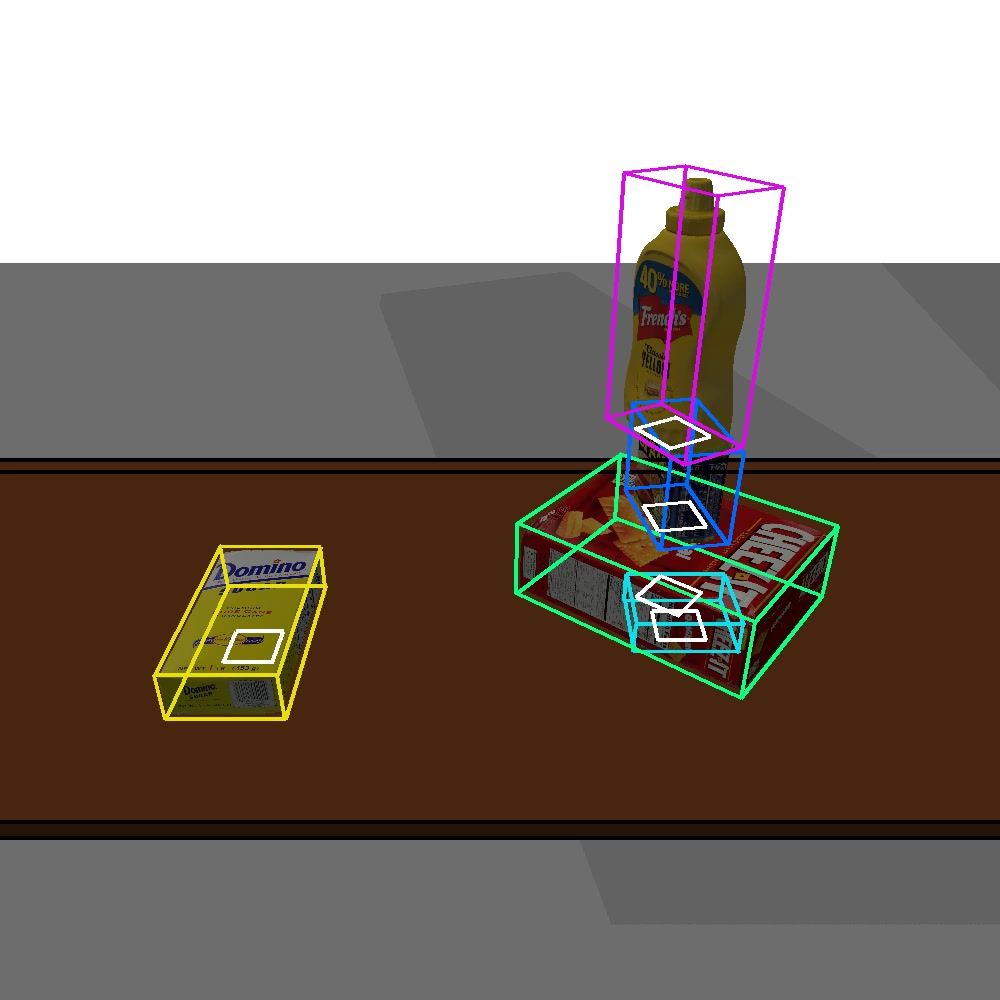
\includegraphics[scale=0.18]{ycbSynthetic1}
  \end{subfigure}%
  \begin{subfigure}[b]{0.45\textwidth}
    \centering
    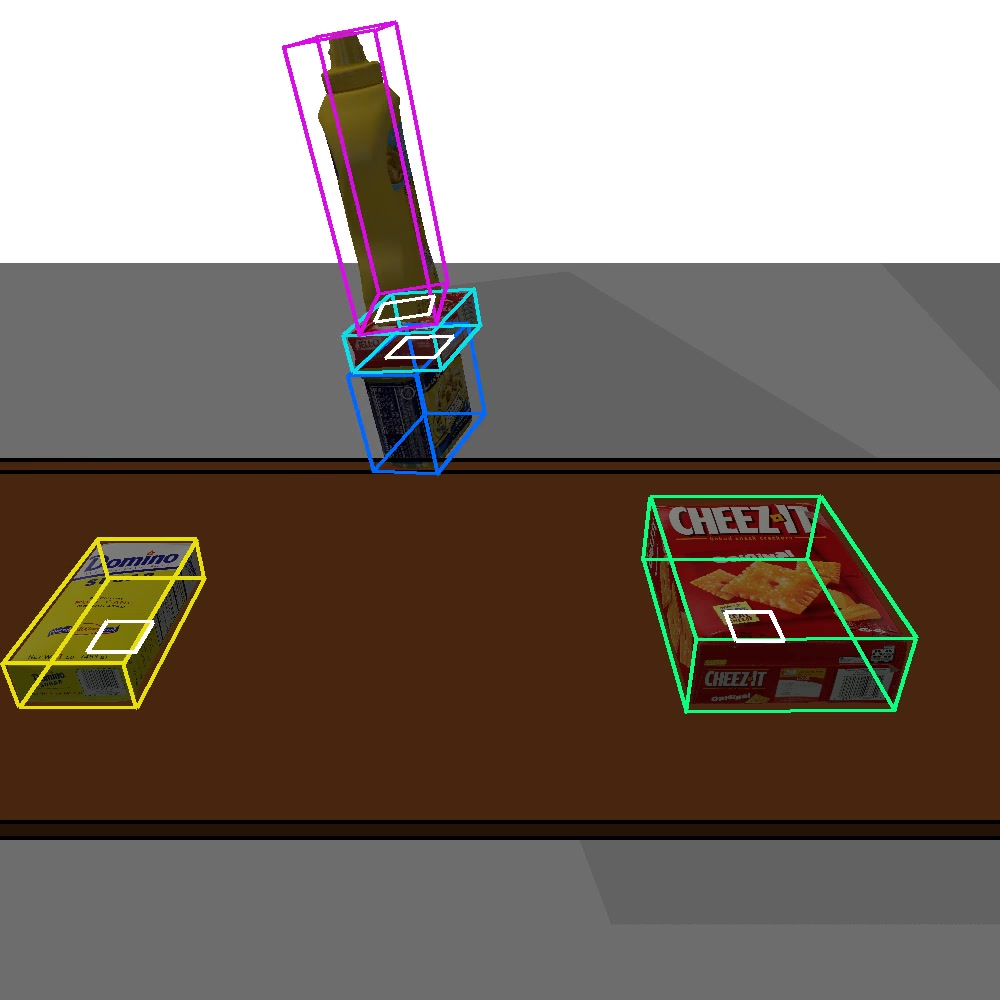
\includegraphics[scale=0.18]{ycbSynthetic2}
  \end{subfigure}
  \begin{subfigure}[b]{0.45\textwidth}
    \centering
    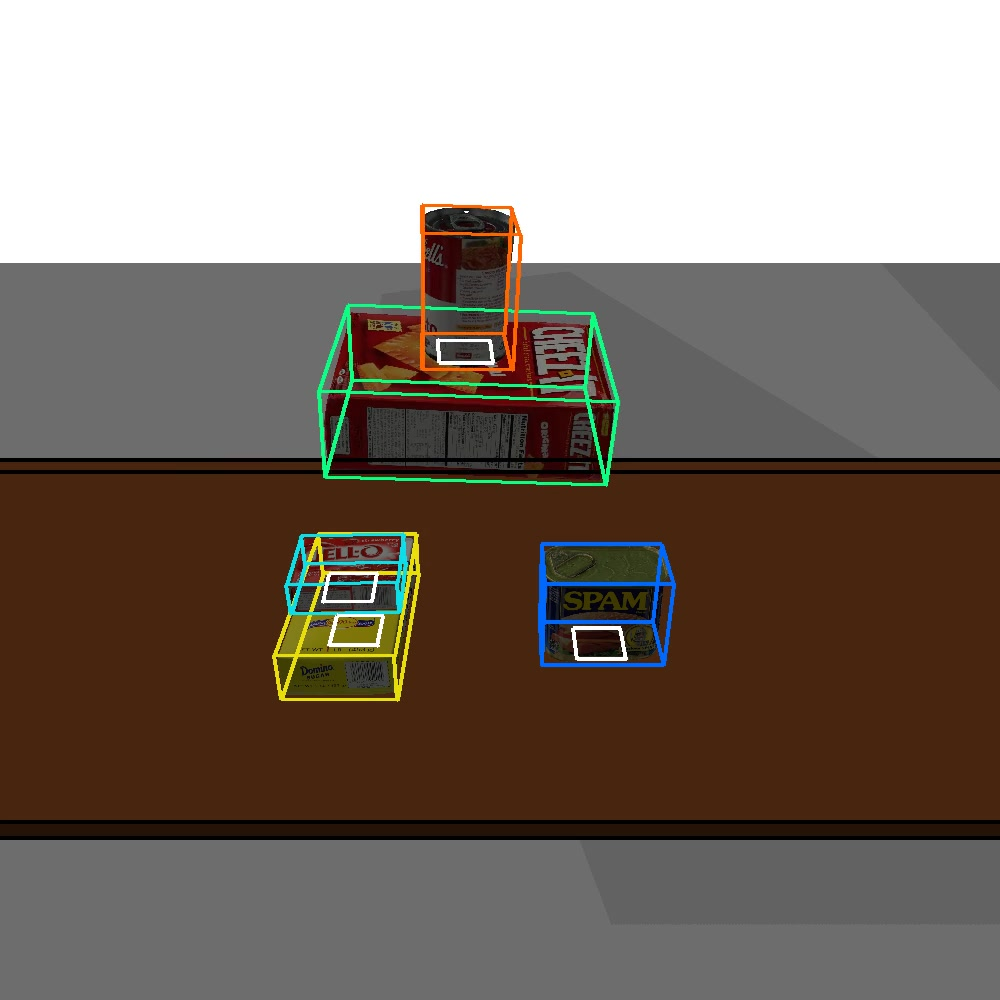
\includegraphics[scale=0.18]{ycbSynthetic3}
  \end{subfigure}%
  \begin{subfigure}[b]{0.45\textwidth}
    \centering
    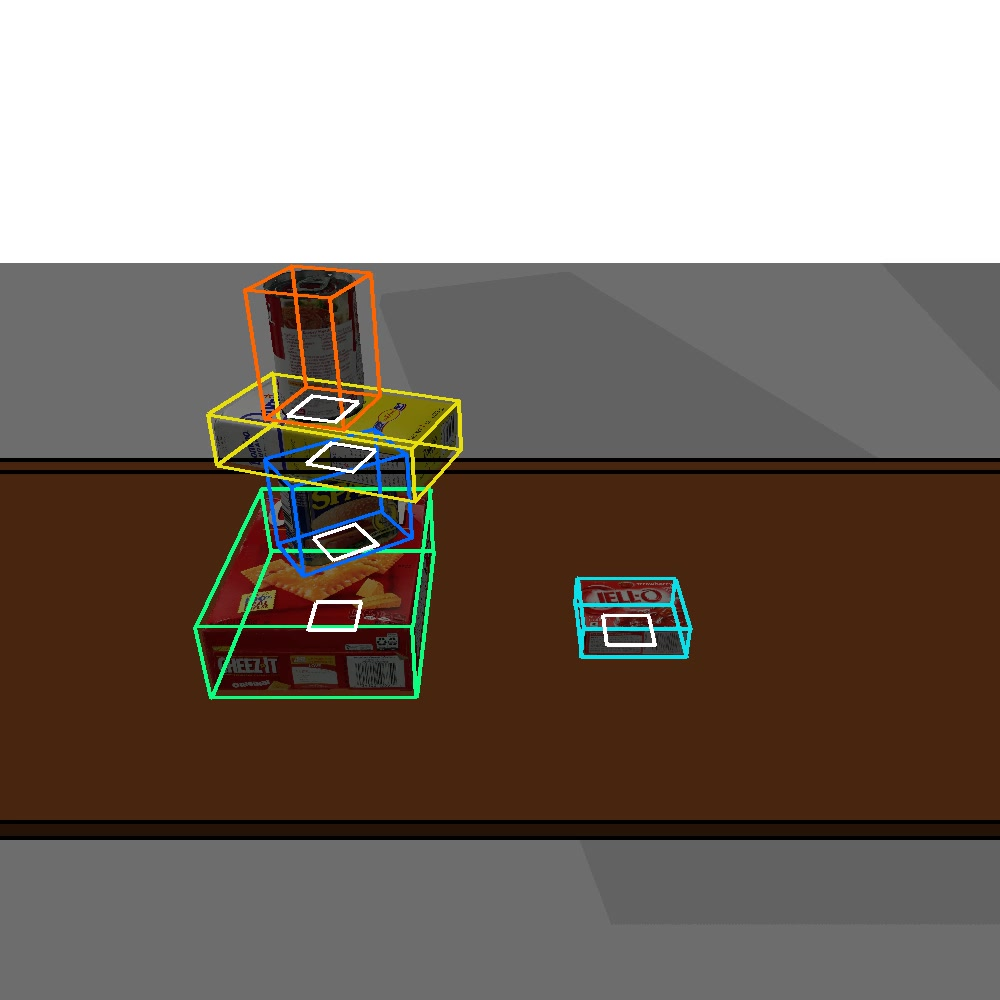
\includegraphics[scale=0.18]{ycbSynthetic4}
  \end{subfigure}
  \caption{
    Synthetic scenes generated using the GenSceneGraphs library in simulated dim light.
    The colored wireframe bounding boxes represent objects in the scene graph, and the white boxes represent contact edges (see Chapter~\ref{chapter3} for more detail on how this visualization was produced).
  }
  \label{fig:syntheticYCBScene}
\end{figure}

Our scene graph abstraction is concretely implemented as a part of the GenSceneGraphs library.
This library provides facilities for constructing and manipulating scene graphs composed of objects that can be rendered in a synthetic view.
Figure~\ref{syntheticYCBScene} shows a variety of example scenes generated using this library; each visualized scene has an underlying scene graph representation that captures all relevant information.
As such, these rendered scenes show an intuitive view of what our information our representation captures.


\subsection{Real YCB Objects on a Physical Tabletop}
\begin{figure}[H]
  \begin{subfigure}[b]{0.45\textwidth}
    \centering
    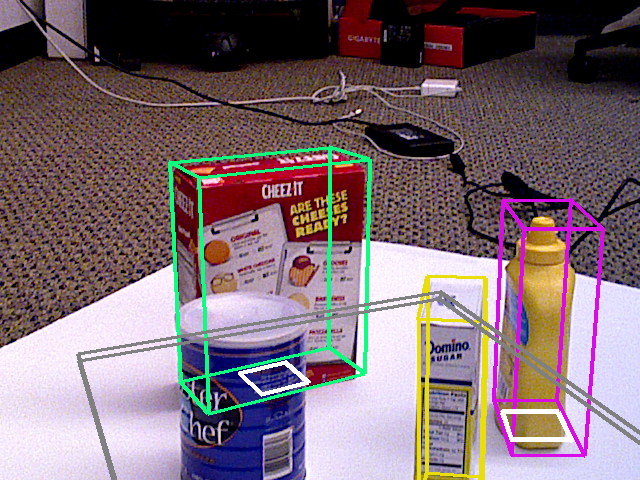
\includegraphics[scale=0.3]{ycbVideoGroundTruth}
    \caption{
      YCB-Video Ground Truth
    }
  \end{subfigure}%
  \begin{subfigure}[b]{0.45\textwidth}
    \centering
    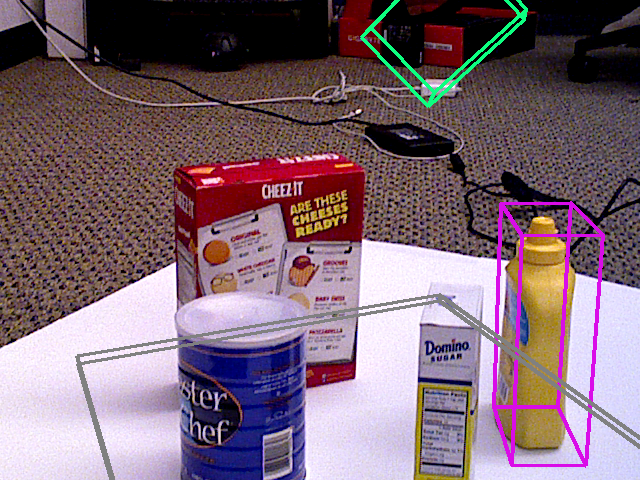
\includegraphics[scale=0.3]{ycbVideoDope}
    \caption{
      YCB-Video nVidia DOPE
    }
  \end{subfigure}
  \begin{subfigure}[b]{0.45\textwidth}
    \centering
    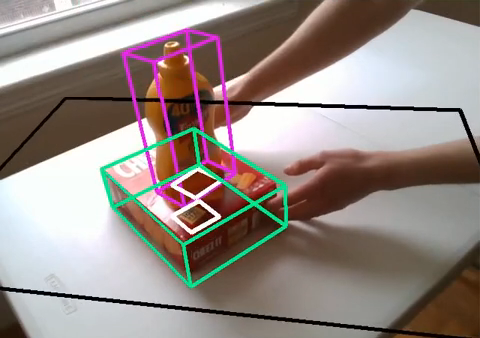
\includegraphics[scale=0.4]{inhouseGroundTruth}
    \caption{
      In-House Dataset
    }
  \end{subfigure}%
  \begin{subfigure}[b]{0.45\textwidth}
    \centering
    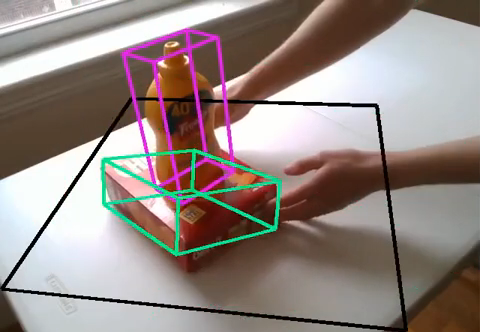
\includegraphics[scale=0.4075]{inhouseDope}
    \caption{
      In-House Dataset nVidia DOPE
    }
  \end{subfigure}
  \caption{
    Example data from real-world scenes containing objects from the YCB dataset.
    (a) and (c) show the underlying latent scene graph.
    (b) and (d) show observed inaccurate pose estimates generated from the nVidia DOPE detector. (b) in particular demonstrates the types of catastrophic detection and localization errors that deep neural networks can exhibit.
  }
  \label{fig:realWorldSceneGraphs}
\end{figure}

Our scene graph representation can be used to represent information about real-world scenes as well.
Figure~\ref{fig:realWorldSceneGraphs} shows how scene graphs can represent the underlying poses and geometric relationships between objects in the real world.
In contrast to the synthetic scenes, the real world contains a much larger variety and range of extraneous variables, that inject noise into visual perception systems and make inference more difficult.
Deep neural networks have shown incredibly promise in real-world object perception.
However, neural networks struggle with robustness and generalization, and the presence of occluders, or even unfamiliar objects, can cause them to fail, as Figure~\ref{fig:realWorldSceneGraphs} also shows.
Our scene graph model was designed with the goal of filtering noisy visual perception systems, and enhancing them with structured information, by inferring the underlying scene graph representation from a set of noisy bottom-up detections.
